\documentclass[11pt]{article}
\usepackage{graphicx} % Required for inserting images
\usepackage{wrapfig}
\usepackage{color}
\usepackage{titlesec}
\usepackage[
    pdfauthor={Eric Van Clepper},
    pdftitle={Chemical feedback of planet formation},
    hidelinks]{hyperref}
\usepackage{amsmath, amssymb}
\newcommand{\link}[1]{{\color{blue}\href{#1}{#1}}}
\providecommand{\tightlist}{\setlength{\itemsep}{0pt}\setlength{\parskip}{0pt}} % for md conversion

\usepackage[margin=0.5in,headsep=0.2in]{geometry}
% \setlength{\headsep}{0.5in}

\usepackage{fancyhdr}
\pagestyle{fancy}
\fancyhf{}
\fancyhead[L]{Eric Van Clepper}
% \fancyhead[C]{\textbf{Chemical feedback of planet formation}}
% \renewcommand{\headrulewidth}{0pt}

% Pandoc CSL reference formatting (correct definitions)
\newlength{\cslhangindent}
\setlength{\cslhangindent}{1.5em}
\newenvironment{CSLReferences}[2]
  {\setlength{\parindent}{0pt}%
   \setlength{\leftskip}{0pt}%
   \setlength{\parskip}{0pt}%
  }
  {}
\newcommand{\CSLBlock}[1]{#1\hfill\break}
\newcommand{\CSLLeftMargin}[1]{\parbox[t]{\cslhangindent}{#1}}
\newcommand{\CSLRightInline}[1]{#1}
\newcommand{\CSLIndent}[1]{\hspace{\cslhangindent}#1}

% section info
\titleformat{\section}
    {\normalfont\bfseries} % formatting
    {}{0em}{} % section number, spacing, code before text
\titleformat{\subsection}
    {\normalfont\bfseries}
    {}{10em}{}
\titlespacing*{\section} % command
{0em}{0.5em}{0em} % left, before, after
\titlespacing*{\subsection}
{10em}{0.5em}{0em}

\usepackage{placeins}
\let\Oldsection\section
\renewcommand{\section}{\FloatBarrier\Oldsection}


\begin{document}
\begin{center}
    \textbf{Chemical feedback of planet formation}
\end{center}
\vspace{-0.5em}

\noindent Despite detections of over 6,000 planets orbiting other
stars\footnote{https://exoplanetarchive.ipac.caltech.edu}, what the
composition of these planets may be, and what that means for the
possibility of life, remains a mystery. My research addresses the
pivotal question: \textit{How}

\begin{wrapfigure}[21]{l}{0.33\textwidth}
    \vspace{-1em}
    \label{fig:disk_cartoon}
    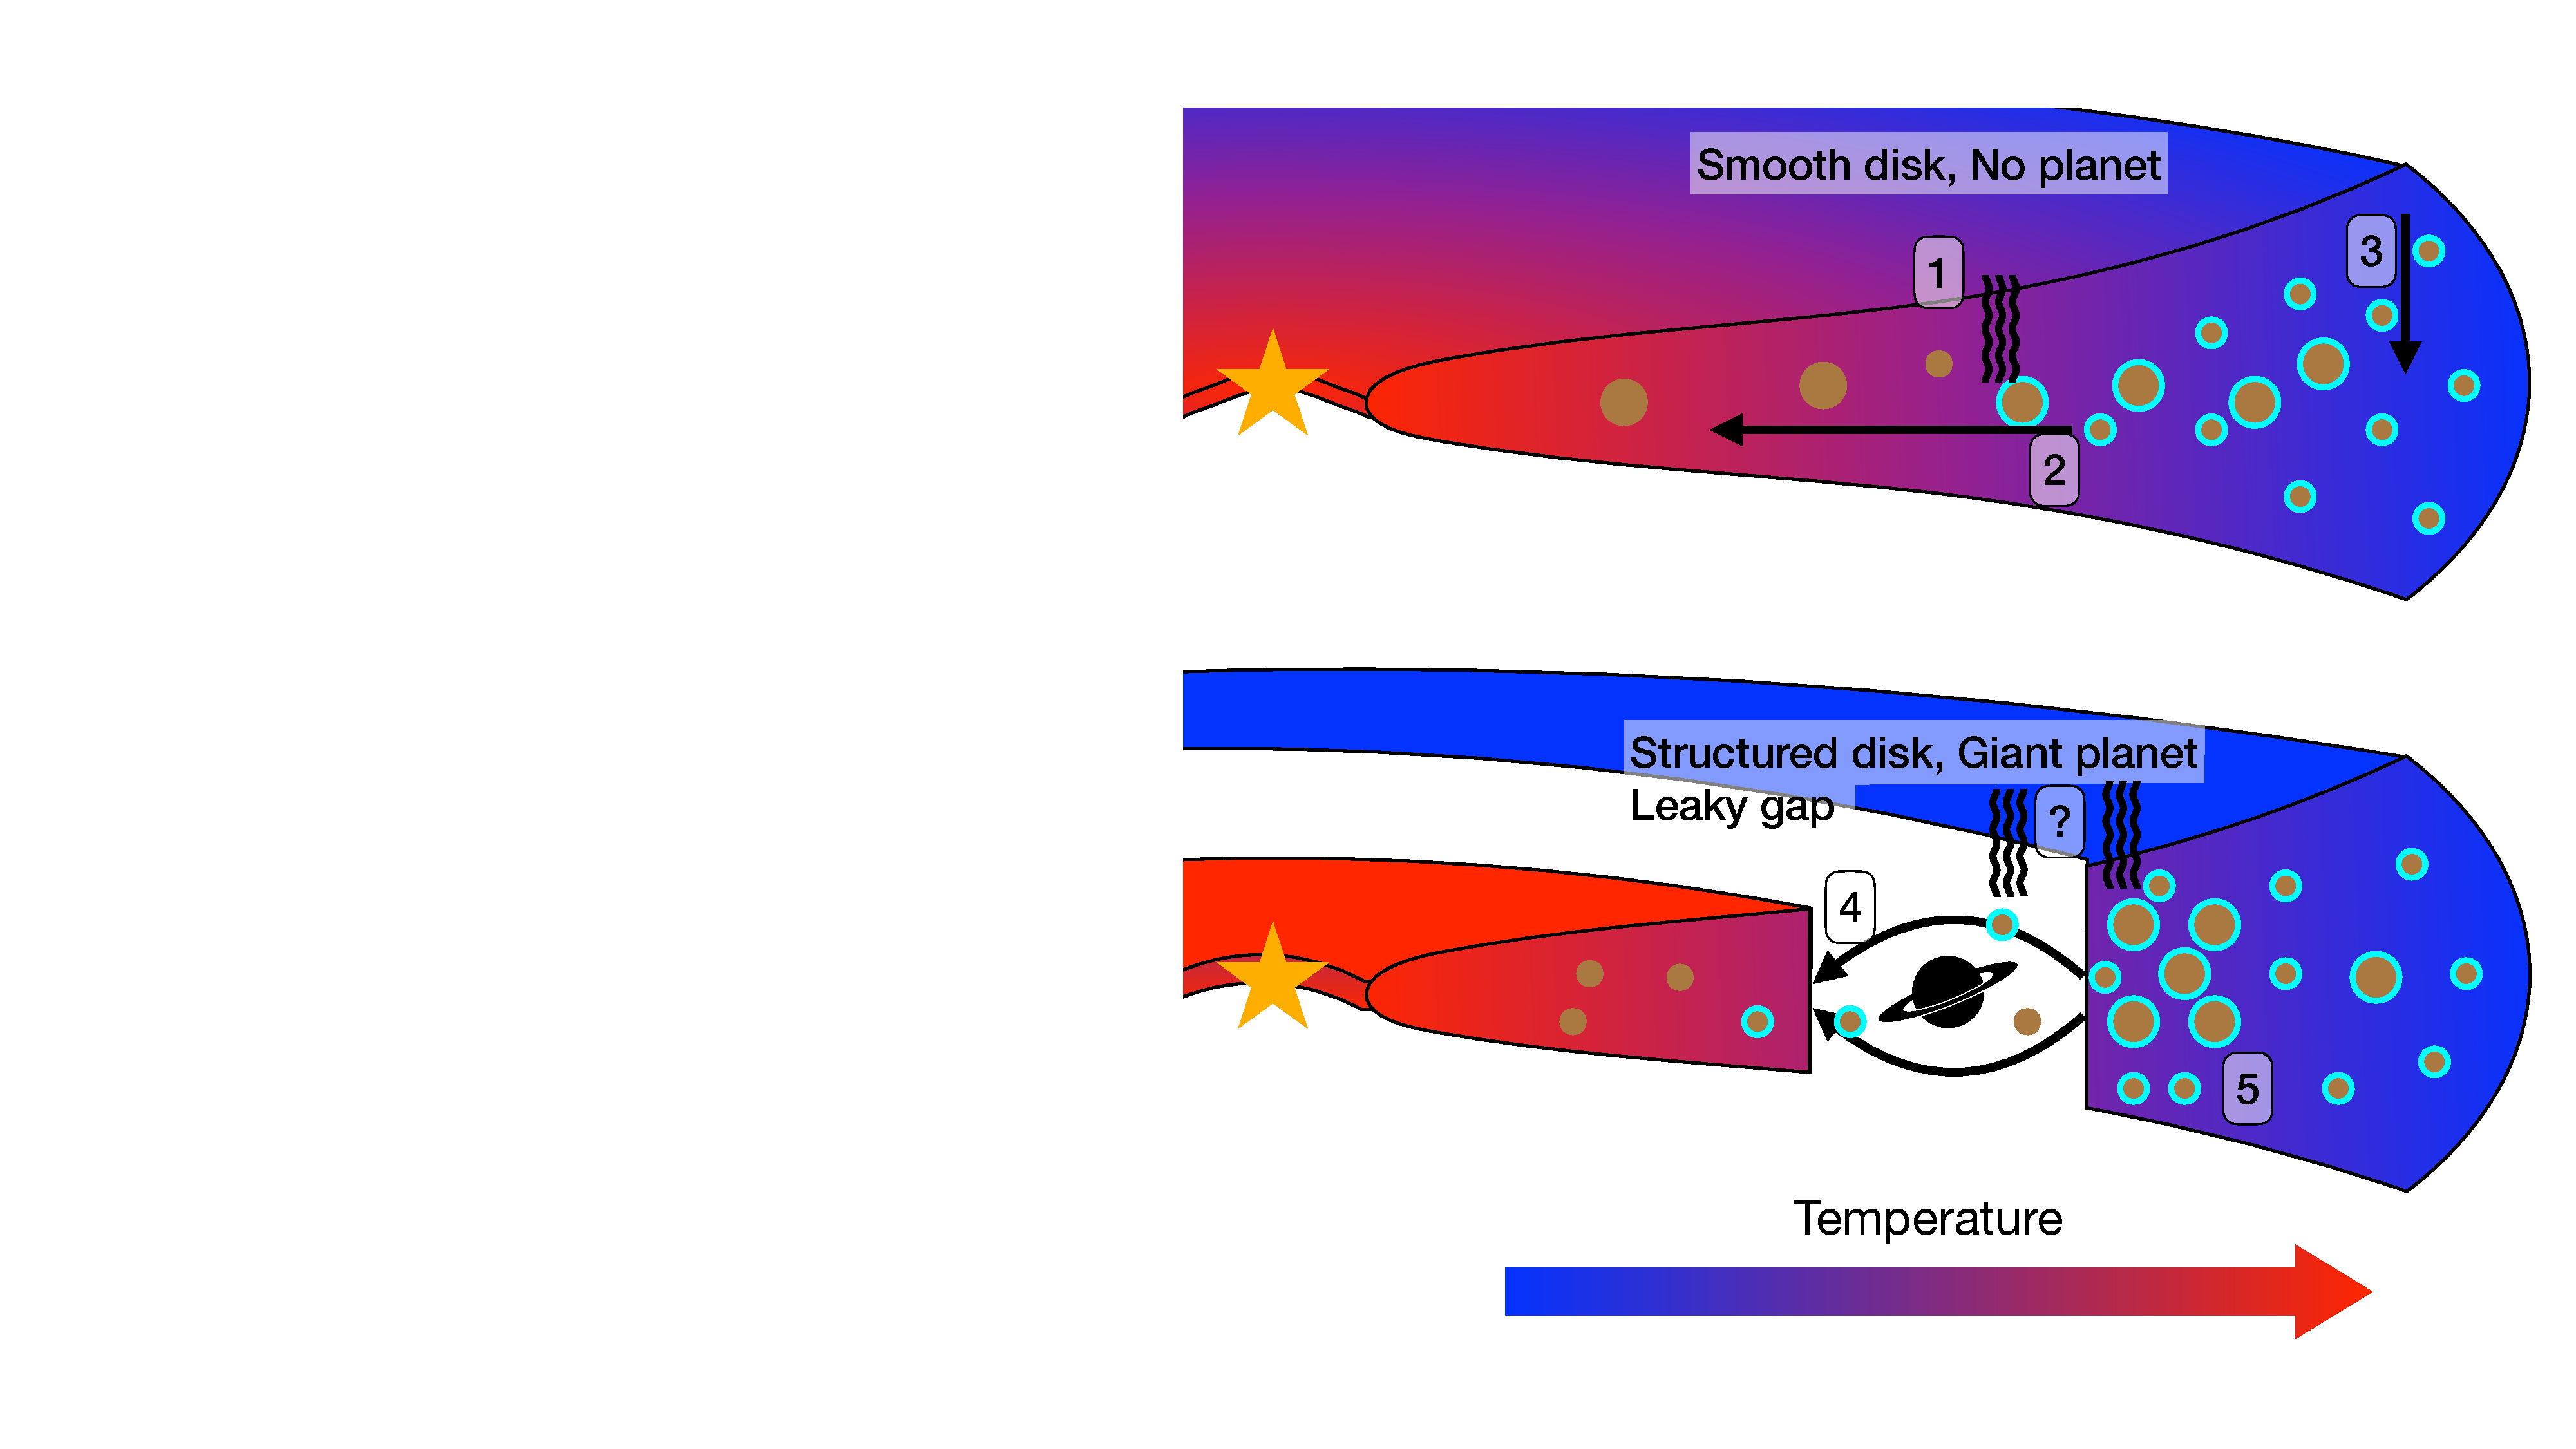
\includegraphics[width=0.33\textwidth]{/Users/ericvc/Documents/Postdocs/disk_stacked_alt.pdf}
    \vspace{-2em}
    \caption{Example disks with and without a giant planet. In the absence of a planet, dust grains are expected to (1) sublimate ice, (2) drift radially inwards, (3) grow and settle. A giant planet however, may lead to (4) selective inward filtering of grains and (5) dust pile-ups in the disk.}
\end{wrapfigure}

\noindent\textit{do growing planets alter the chemical environment of planet formation?}

\hypertarget{background}{%
\section{Background}\label{background}}

As gas and dust collapse from the interstellar medium to form a young
protostar, a small fraction of the total mass creates a protoplanetary
disk (PPD), a ring of gas and dust from which planets will form. While
it has long been assumed that planets reflect the composition of the
disk in which they form (e.g. {[}1{]}), recent observations of molecular
line emission from protoplanetary disks have shown that not only are
these disks highly dynamic {[}2{]}, but also regions of active, and yet
unexplained, chemistry {[}3{]}. One attractive explanation is the the
presence of giant planets, similar to Jupiter in our solar system, which
can have dramatic effects on the gas and dust distribution (Fig 1).
\textbf{These dynamic effects may be altering not only their own birth
environment, but also the subsequent formation of other planets around
the same star.}

Despite recent advancements in our understanding of the chemical
composition of PPDs, exoplanets, and bodies in our own solar system, we
still lack a comprehensive theoretical framework connecting the chemical
evolution PPDs to the planets that form within. Throughout my PhD, I
have pioneered theoretical modeling techniques to examine the dynamic
and chemical connections between the gas, dust, and planets withing a
PPD {[}4,5{]}. As a Miller Fellow at Berkeley I will continue this work
to model the dynamic chemical environments of the PPD and connect
planetary compositions to their natal disk.

\hypertarget{research-approach}{%
\section{Research Approach}\label{research-approach}}

I will use a combination of \textbf{advanced 3D hydrodynamic models}
with Monte Carlo particle integration to track the trajectories of ice
covered grains through a PPD containing a giant planet. Not only do
these small grains set the available temperature and UV radiation
throughout the disk, but their surfaces provide important sites of
grain-surface chemistry. Simple molecules present on the ice, such as
water and carbon dioxide, can react with radiation from the host star
creating complex carbohydrates {[}6{]}. Too much radiation, however, can
sublimate ice or destroy these complex molecules all together. With my
combined dynamic and chemical models I will be able to constrain this
processing of volatile ices, and what this means for the possible
delivery of life-relevant molecules to planets in our solar system and
beyond.

Following on this, I will track both the dust and gas-phase chemistry
together, modeling \textbf{coupled chemical evolution} in a
self-consistent manner for the first time. Current disk models assume
static disks, which cannot differentiate between chemical versus
dynamical effects. My 3D dynamic models will inform the dust evolution
in 2D chemical models, creating a new step forward for accurate disk
chemical modeling and providing new insight for interpreting disk
observations.

Finally, these combined chemistry and dynamic models for disks
containing planets will allow me to \textbf{directly link planet
compositions to disk conditions}. Even if these planets do not mirror
the observed disk composition, the detection of tracer molecular species
in the disk may tell us something about the planets forming inside. I
will create the self-consistent modelling framework necessary to know
the compositions of these yet undetected planets and if they are indeed
hospitable for life.

\hypertarget{references}{%
\section*{References}\label{references}}
\addcontentsline{toc}{section}{References}

\hypertarget{refs}{}
\begin{CSLReferences}{0}{0}
\leavevmode\vadjust pre{\hypertarget{ref-oberg_EFFECTS_2011}{}}%
\CSLLeftMargin{{[}1{]} }%
\CSLRightInline{\href{https://doi.org/10.1088/2041-8205/743/1/L16}{Öberg,
K. I., Murray-Clay, R. \& Bergin, E. A. 2011, \emph{ApJ}, \textbf{743},
L16}.}
\leavevmode\vadjust pre{\hypertarget{ref-andrews_Disk_2018}{}}%
\CSLLeftMargin{{[}2{]} }%
\CSLRightInline{\href{https://doi.org/10.3847/2041-8213/aaf741}{Andrews,
S. M., Huang, J., Pérez, L. M., \emph{et al.} 2018, \emph{ApJ},
\textbf{869}, L41}.}
\leavevmode\vadjust pre{\hypertarget{ref-oberg_Molecules_2021}{}}%
\CSLLeftMargin{{[}3{]} }%
\CSLRightInline{\href{https://doi.org/10.3847/1538-4365/ac1432}{Öberg,
K. I., Guzmán, V. V., Walsh, C., \emph{et al.} 2021, \emph{ApJS},
\textbf{257}, 1}.}
\leavevmode\vadjust pre{\hypertarget{ref-vanclepper_Chemical_2022}{}}%
\CSLLeftMargin{{[}4{]} }%
\CSLRightInline{\href{https://doi.org/10.3847/1538-4357/ac511b}{Van
Clepper, E., Bergner, J. B., Bosman, A. D., \emph{et al.} 2022,
\emph{ApJ}, \textbf{927}, 206}.}
\leavevmode\vadjust pre{\hypertarget{ref-vanclepper_Threedimensional_2025}{}}%
\CSLLeftMargin{{[}5{]} }%
\CSLRightInline{\href{https://doi.org/10.3847/1538-4357/ada8a4}{Van
Clepper, E., Price, E. \& Ciesla, F. J. 2025, \emph{ApJ}, \textbf{980},
201}.}
\leavevmode\vadjust pre{\hypertarget{ref-bergner_Ice_2021}{}}%
\CSLLeftMargin{{[}6{]} }%
\CSLRightInline{\href{https://doi.org/10.3847/1538-4357/ac0fd7}{Bergner,
J. B. \& Ciesla, F. 2021, \emph{ApJ}, \textbf{919}, 45}.}

\end{CSLReferences}
\end{document}